\mysubsubsection{Layered Depthmap}

\begin{figure}[tb]
  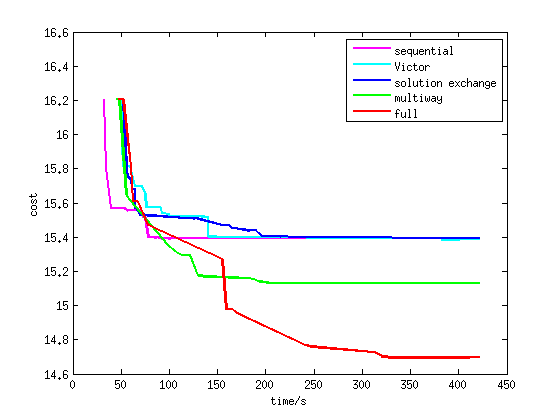
\includegraphics[width=\columnwidth]{figure/layered_depthmap_convergence.png}
  \caption{The energy minimization process for layered depthmap estimation of different methods. Multi-way fusion is shown to be more effectvie than binary fusion in this problem setting.}\label{fig:layered_depthmap_convergence}
\end{figure}
\begin{figure}[tb]
  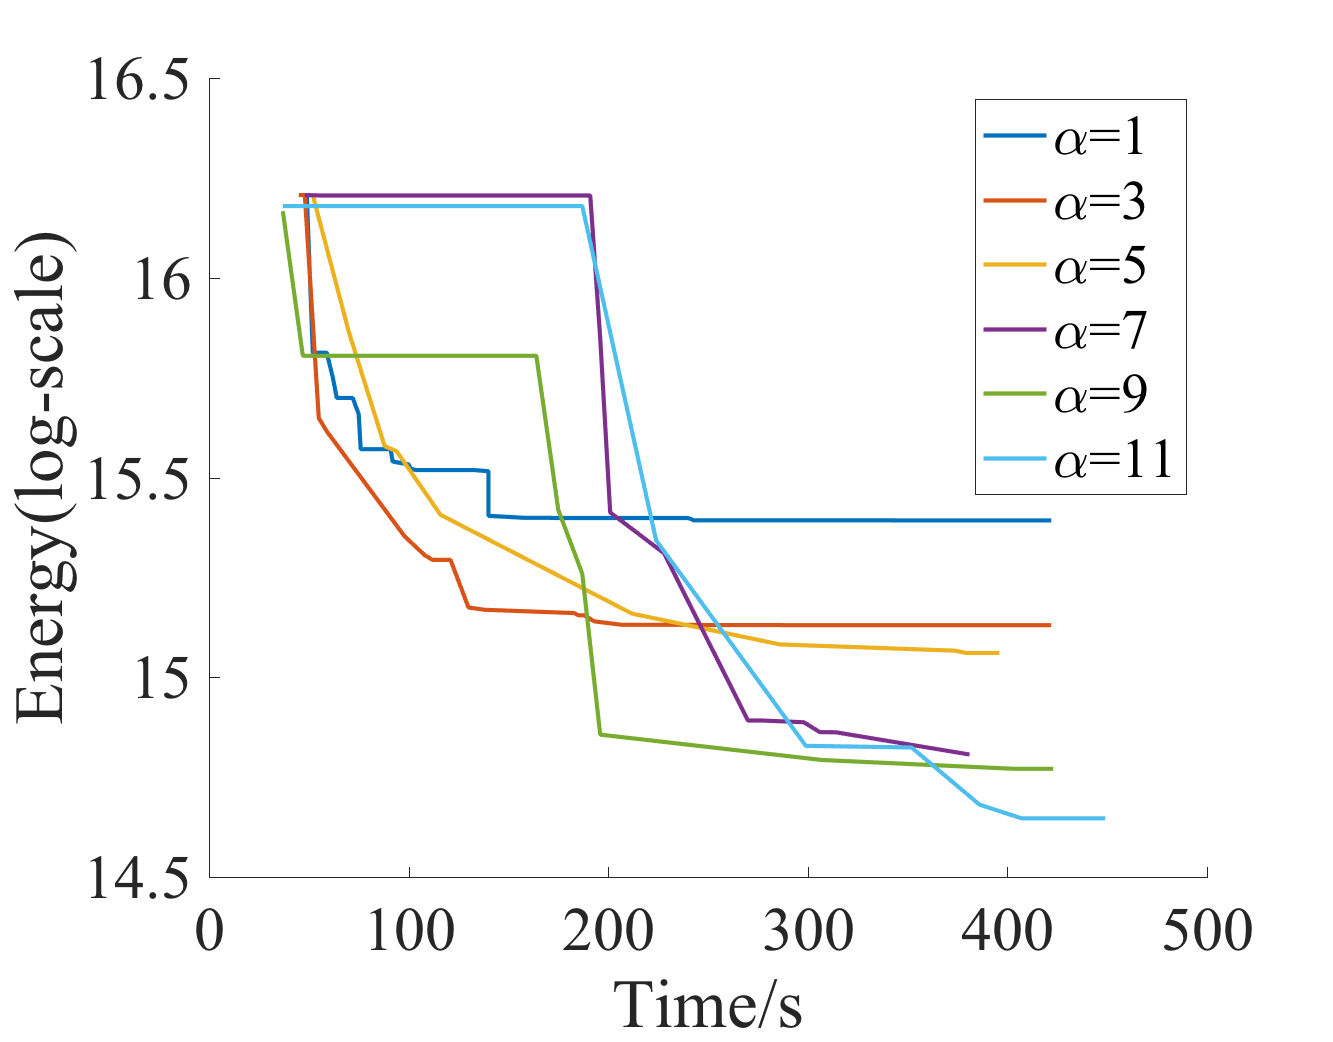
\includegraphics[width=\columnwidth]{figure/layered_depthmap_by_alpha.png}
  \caption{The energy minimization process for layered depthmap estimation with different $\alpha$ values. Multi-way fusion generally performs better than binary fusion, but the optimization becomes harder for using more ways in each step.}\label{fig:layered_depthmap_by_alpha}
\end{figure}

We did our experiments on ours\_1 dataset in~\cite{layered_depthmap}. We plot the energy minimization process in figure \ref{fig:layered_depthmap_convergence}. From the plot, we can see that, Fusion Move, Parallel Fusion Move, and SF-MF all stalk at a high energy state. The reason is binary fusion of solution proposals (either from others or self) is too limited to contain a lower energy state due to the complexity of the problem itself. Only when multi-way fusion which explores much larger solution space is used (in SF-SS and SF), it becomes possible for the energy to further decrease. This coincides with the observation in \cite{layered_depthmap} that binary fusion of proposal solutions is not as powerful as their subspace fusion which is a special form of multi-way fusion here. Note that SF also utilize multi-way fusion for solution sharing so that it performs better than SF-SS which has no solution sharing.

To further explore the effect of multi-way fusion, we use different $\alpha = {1, 3, 7, 15}$ in SF-SS model (disable solution sharing to better observe the effect of multi-way fusion) while keeping other parameters the same and plot the energy minimization process in figure \ref{fig:layered_depthmap_by_alpha}. We can see that as the number of ways to fuse becomes larger, each fusion step takes longer time, but the chance of finding a lower energy state increases.


